\paragraph{Conflict Serializable Schedules}

\begin{itemize}
\item Two schedules are \textbf{conflict equivalent} if:
  \begin{itemize}
  \item involve the same actions of the same transactions
  \item every pair of conflicting actions is ordered the
    same way
  \item two actions are called \textbf{conflicting} if they access
    the same object and one of them is a write
  \end{itemize}

\item Schedule S is \textbf{conflict serializable} if S is conflict
  equivalent to some serial schedule
\end{itemize}

\paragraph{Example: Schedule not conflict serializable}
\begin{itemize}
\item the cycle in the graph reveals the problem. The
  output of T1 depends on T2, and vice-versa.
\end{itemize}

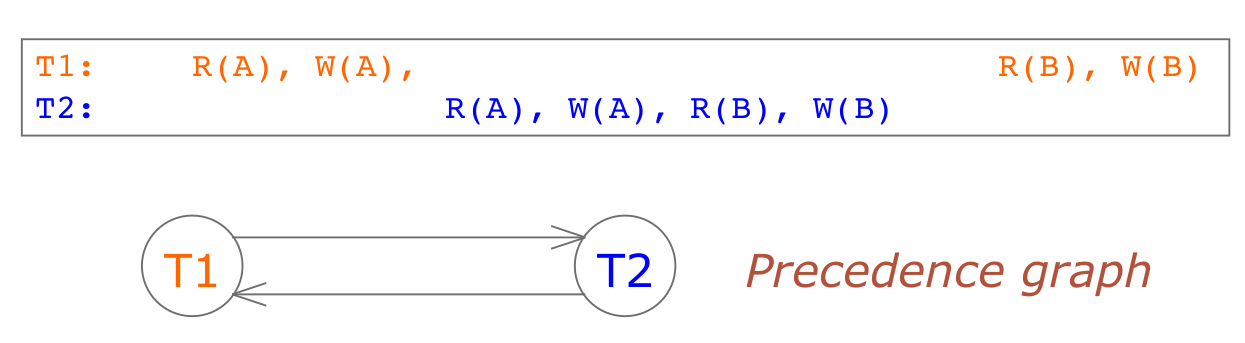
\includegraphics[scale=0.15]{graphics/not-conflict-serializable.png}


\paragraph{Precedence Graph}
\begin{itemize}
\item \textbf{Precedence graph:} One node per Xact; edge from
  $T_i$ to $T_j$ if operation in $T_j$ conflicts with earlier operation
  in $T_i$

\item \textbf{Theorem:} Schedule is conflict serializable if
  and only if its precedence graph is acyclic
\item Strict 2PL only results in conflict serializable schedules
  \begin{itemize}
  \item Precedence graph is always acyclic
  \end{itemize}
\end{itemize}

\paragraph{View serializability}
\begin{itemize}
\item Schedules S1 and S2 are \textbf{view equivalent} if:
  \begin{itemize}
  \item $T_i$ reads initial value of A in S1, then $T_i$ also
    reads initial value of A in S2
  \item if $T_i$ reads a value of A written by $T_j$ in S1, then
    $T_i$ also reads value of A written by $T_j$ in S2
  \item If $T_i$ writes final value of A in S1, then $T_i$ also
    writes final value of A in S2
  \end{itemize}
\end{itemize}


\paragraph{Deadlocks}
\begin{itemize}
\item Deadlock: Cycle of transactions waiting for locks to be
  released by each other

\item Two ways of dealing with deadlocks:
  \begin{itemize}
  \item Deadlock prevention
  \item Deadlock detection
  \end{itemize}
\end{itemize}

\paragraph{Deadlock Prevention}
\begin{itemize}
\item Assign priorities based on timestamps
\item Lower timestamps get higher priority, i.e.,
  older transactions get prioritized
\item Assume $T_i$ wants a lock that $T_j$ holds. Two
  policies are possible:
  \begin{itemize}
  \item Wait-Die: If $T_i$ has higher priority, $T_i$ waits for
    $T_j$; otherwise $T_i$ aborts
  \item Wound-wait: If $T_i$ has higher priority, $T_j$ aborts;
    otherwise $T_i$ waits
  \end{itemize}

\item If a transaction re-starts, make sure it has its
  original timestamp
\end{itemize}

\paragraph{Deadlock Detection}
\begin{itemize}
\item Create a \textbf{waits-for graph}:
  \begin{itemize}
  \item Nodes are transactions
  \item There is an edge from $T_i$ to $T_j$ if $T_i$ is waiting
    for $T_j$ to release a lock
  \end{itemize}

\item Periodically check for cycles in the waits-for graph
\end{itemize}

\paragraph{The Problems with Locking}
\begin{itemize}
\item Locking is a pessimistic approach in which conflicts are
  prevented
\item Disadvantages:
  \begin{itemize}
  \item Lock management overhead
  \item Deadlock detection/resolution necessary
  \item Lock contention for heavily used objects
  \end{itemize}

\item We must devise a way to
  \textbf{{\color{red} enforce serializability}}, without
  destroying concurrency
\item Two approaches:
  \begin{itemize}
  \item prevent violations → locking
  \item fix violations → aborts
  \end{itemize}
\end{itemize}

\paragraph{Optimistic CC: Kung-Robinson Model}
\begin{itemize}
\item optimistic approach based on aborts
\item Xacts have three phases
\item \textbf{READ:} Xacts read from the database, but
  make changes to private copies of the objects
\item \textbf{VALIDATE:} check for conflicts
\item \textbf{WRITE:} make local copies of changes public
\end{itemize}

\paragraph{Validation}
\begin{itemize}
\item Test conditions that are \textbf{sufficient} to ensure
  that no conflict occurred
\item Each Xact is assigned a numeric id
  \begin{itemize}
  \item simply use a \textbf{timestamp}
  \end{itemize}

\item Xact ids assigned at end of READ phase, just before
  validation begins

\item ReadSet($T_i$): Set of objects read by Xact $T_i$
\item WriteSet($T_i$): Set of objects modified by $T_i$
\end{itemize}

\paragraph{Test 1}
\begin{itemize}
\item For all $i$ and $j$ such that $T_i < T_j$, check that
  $T_i$ completes before $T_j$ begins
\end{itemize}

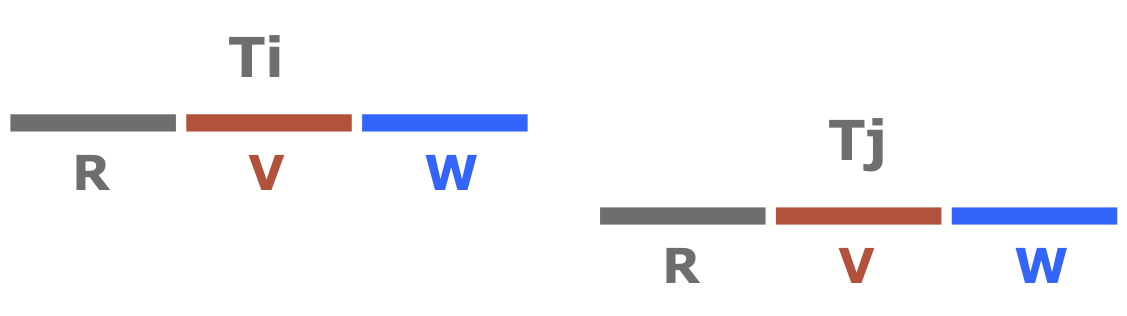
\includegraphics[scale=0.15]{graphics/Test-1.png}

\paragraph{Test 2}
\begin{itemize}
\item For all $i$ and $j$ such that $T_i < T_j$, check that:
  \begin{itemize}
  \item $T_i$ completes before $T_j$ begins its Write phase
  \item WriteSet($T_i$) $\cap$ ReadSet($T_j$) is empty
  \end{itemize}
\end{itemize}

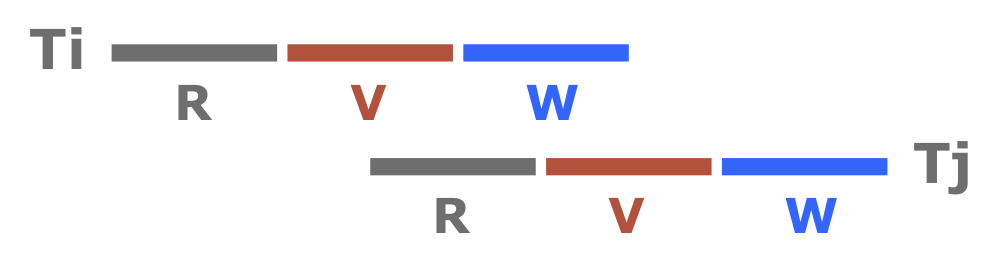
\includegraphics[scale=0.15]{graphics/Test-2.png}

\paragraph{Test 3}
\begin{itemize}
\item For all $i$ and $j$ such that $T_i < T_j$, check that:
  \begin{itemize}
  \item $T_i$ completes Read phase before $T_j$ does
  \item WriteSet($T_j$) $\cap$ ReadSet($T_J$) is empty
  \item WriteSet($T_i$) $\cap$ WriteSet($T_j$) is empty
  \end{itemize}
\end{itemize}

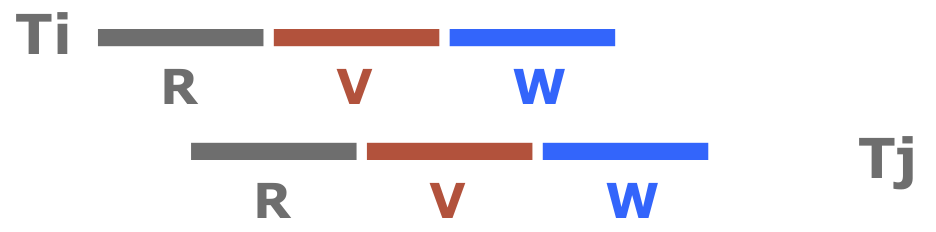
\includegraphics[scale=0.15]{graphics/Test-3.png}


\paragraph{Overheads in Optimistic CC}
\begin{itemize}
\item Must record read/write activity in ReadSet and WriteSet
  per Xact
  \begin{itemize}
  \item must create and destroy these sets as needed
  \end{itemize}

\item Must check for conflicts during validation, and must
  make validated writes ``global''
  \begin{itemize}
  \item Critical section can reduce concurrency
  \item Scheme for making writes global can reduce clustering of
    objects
  \end{itemize}

\item Optimistic CC restarts Xacts that fail validation
  \begin{itemize}
  \item work done so far is wasted; requires clean-up
  \end{itemize}

\item Still, optimistic techniques widely used in
  software transactional memory (STM), main-memory databases
\end{itemize}


\paragraph{Snapshot Isolation}
\begin{itemize}
\item Often databases implement properties that are \textbf{weaker}
  than serializability
\item \textbf{Snapshot isolation}
  \begin{itemize}
  \item \textbf{Snapshots:} Transactions see snapshot as of beginning
    of their execution
  \item \textbf{First Committer Wins:} Conflicting writes to same
    item lead to aborts
  \end{itemize}
\item May lead to \textbf{write skew}
  \begin{itemize}
  \item Database must have at least one doctor on call
  \item Two doctors on call concurrently examine snapshot and see
    exactly each other on call
  \item Doctors update their own records to being on leave
    \begin{itemize}
    \item No writ-write conflicts: different records!
    \end{itemize}
  \item after commits, database has no doctors on call
  \end{itemize}
\end{itemize}
% LocalWords:  Serializable serializable Xact acyclic serializability
% LocalWords:  Kung Xacts ReadSet WriteSet transactional STM
